\documentclass{article}
\usepackage{gensymb}
\usepackage{textcomp}
\usepackage{amsmath}
\usepackage{hyperref}
\usepackage{bookmark}
\usepackage{float} 
\usepackage{graphicx}
\usepackage{makeidx}
\usepackage[letterpaper, total={7.5in, 10in}]{geometry}

\makeindex
\begin{document}
\title{Formal Project Proposal}
\author{Geoffrey Huang and Elias Xu}
\date{\today}
\maketitle
\setlength{\parindent}{0pt}

\section{Description}

We’re planning on analyzing/simulating the oscillations on a ball induced by buoyant force, the force of gravity, and drag. The user would be able to set the ball's (which will be initial suspended inside the surface, this allows for starting position below the water) initial height and velocity (with horizontal and vertical components) and then drop it, which will fall due to gravity (which can also be changed by the user). The user will also be able to set the physical properties of the ball, such as the volume and mass of the ball. The ball will then fall into the liquid with variable properties (with presets like water, mercury, and oil). Then the simulation will show the oscillations of the ball over time, until the ball stops (given drag), which will be a threshold epsilon. The program will measure and graph the system's energy, position of the ball (in the y direction), acceleration, and velocity of the ball, period of the oscillation, and frequency.


\subsection{Formulas / Methodology}

We'll be using VPython's method of splitting up a simulation by dividing up time into little segments, and then updating the ball's net force, acceleration, velocity, and then position.

Before the object hits the water, the only force that should be acting on the ball would be the force of gravity.

$$F = mg$$

After the object hits the water, there would be three forces acting on the ball in the water, one being the gravitational force, another one being the buoyant force, and the third one being the drag force from the water. Again, the force of gravity is represented by $F = mg$, which is still also directed downwards.

The buoyant force will be pointed upwards to the surface, and it's defined as:

$$F_b = -\rho gV$$

Where $g$ is the acceleration due to gravity, $\rho$ is the fluid density of the fluid and $V$ is the volume displaced by the object. Since the ball is not going to be fully submerged all the time, volume must be measured in terms of height submerged, making the formula that we're going to use the formula for the volume of a spherical cap, which is $V = \frac{1}{3}\pi h^2 (3r - h)$, which makes the resulting formula to be.

$$F_b = - \frac{1}{3} \pi \rho g h^2 (3r - h)$$

Finally, the force of drag will be opposed to the force of velocity, and after substituting for the surface area of a cap based on the height submerged, the formula should be:

$$F_{\text{drag}} = \frac{1}{2} C_D \rho v^2 A = \frac{1}{2} C_D \rho v^2 \sqrt{r^2 - (r-h)^2}$$

Where $C_D$ is the drag coefficient, and $A$ is the surface area.

\subsection{Stretch Goals}

We have multiple stretch goals. The first stretch goal would be to apply air resistance to the object, which should be simple enough. This however, should result in a very small change, so I guess another possible object would be to apply a "wind" to the ball, which could mean that we would have to break out of the y-axis, and move to the x-axis. The second goal is to have a ball of substrate/salt and have the ball dissolve as it oscillates, which could be interesting about the oscillations and energy. Then, we could use some parametric motion, such as initial velocity. Finally, our last goal would be to use an asymmetrical object, such as a stick, to model the torques that could be applied.

\section{Screenshot(s)}


\begin{figure}[H]
    \centering
    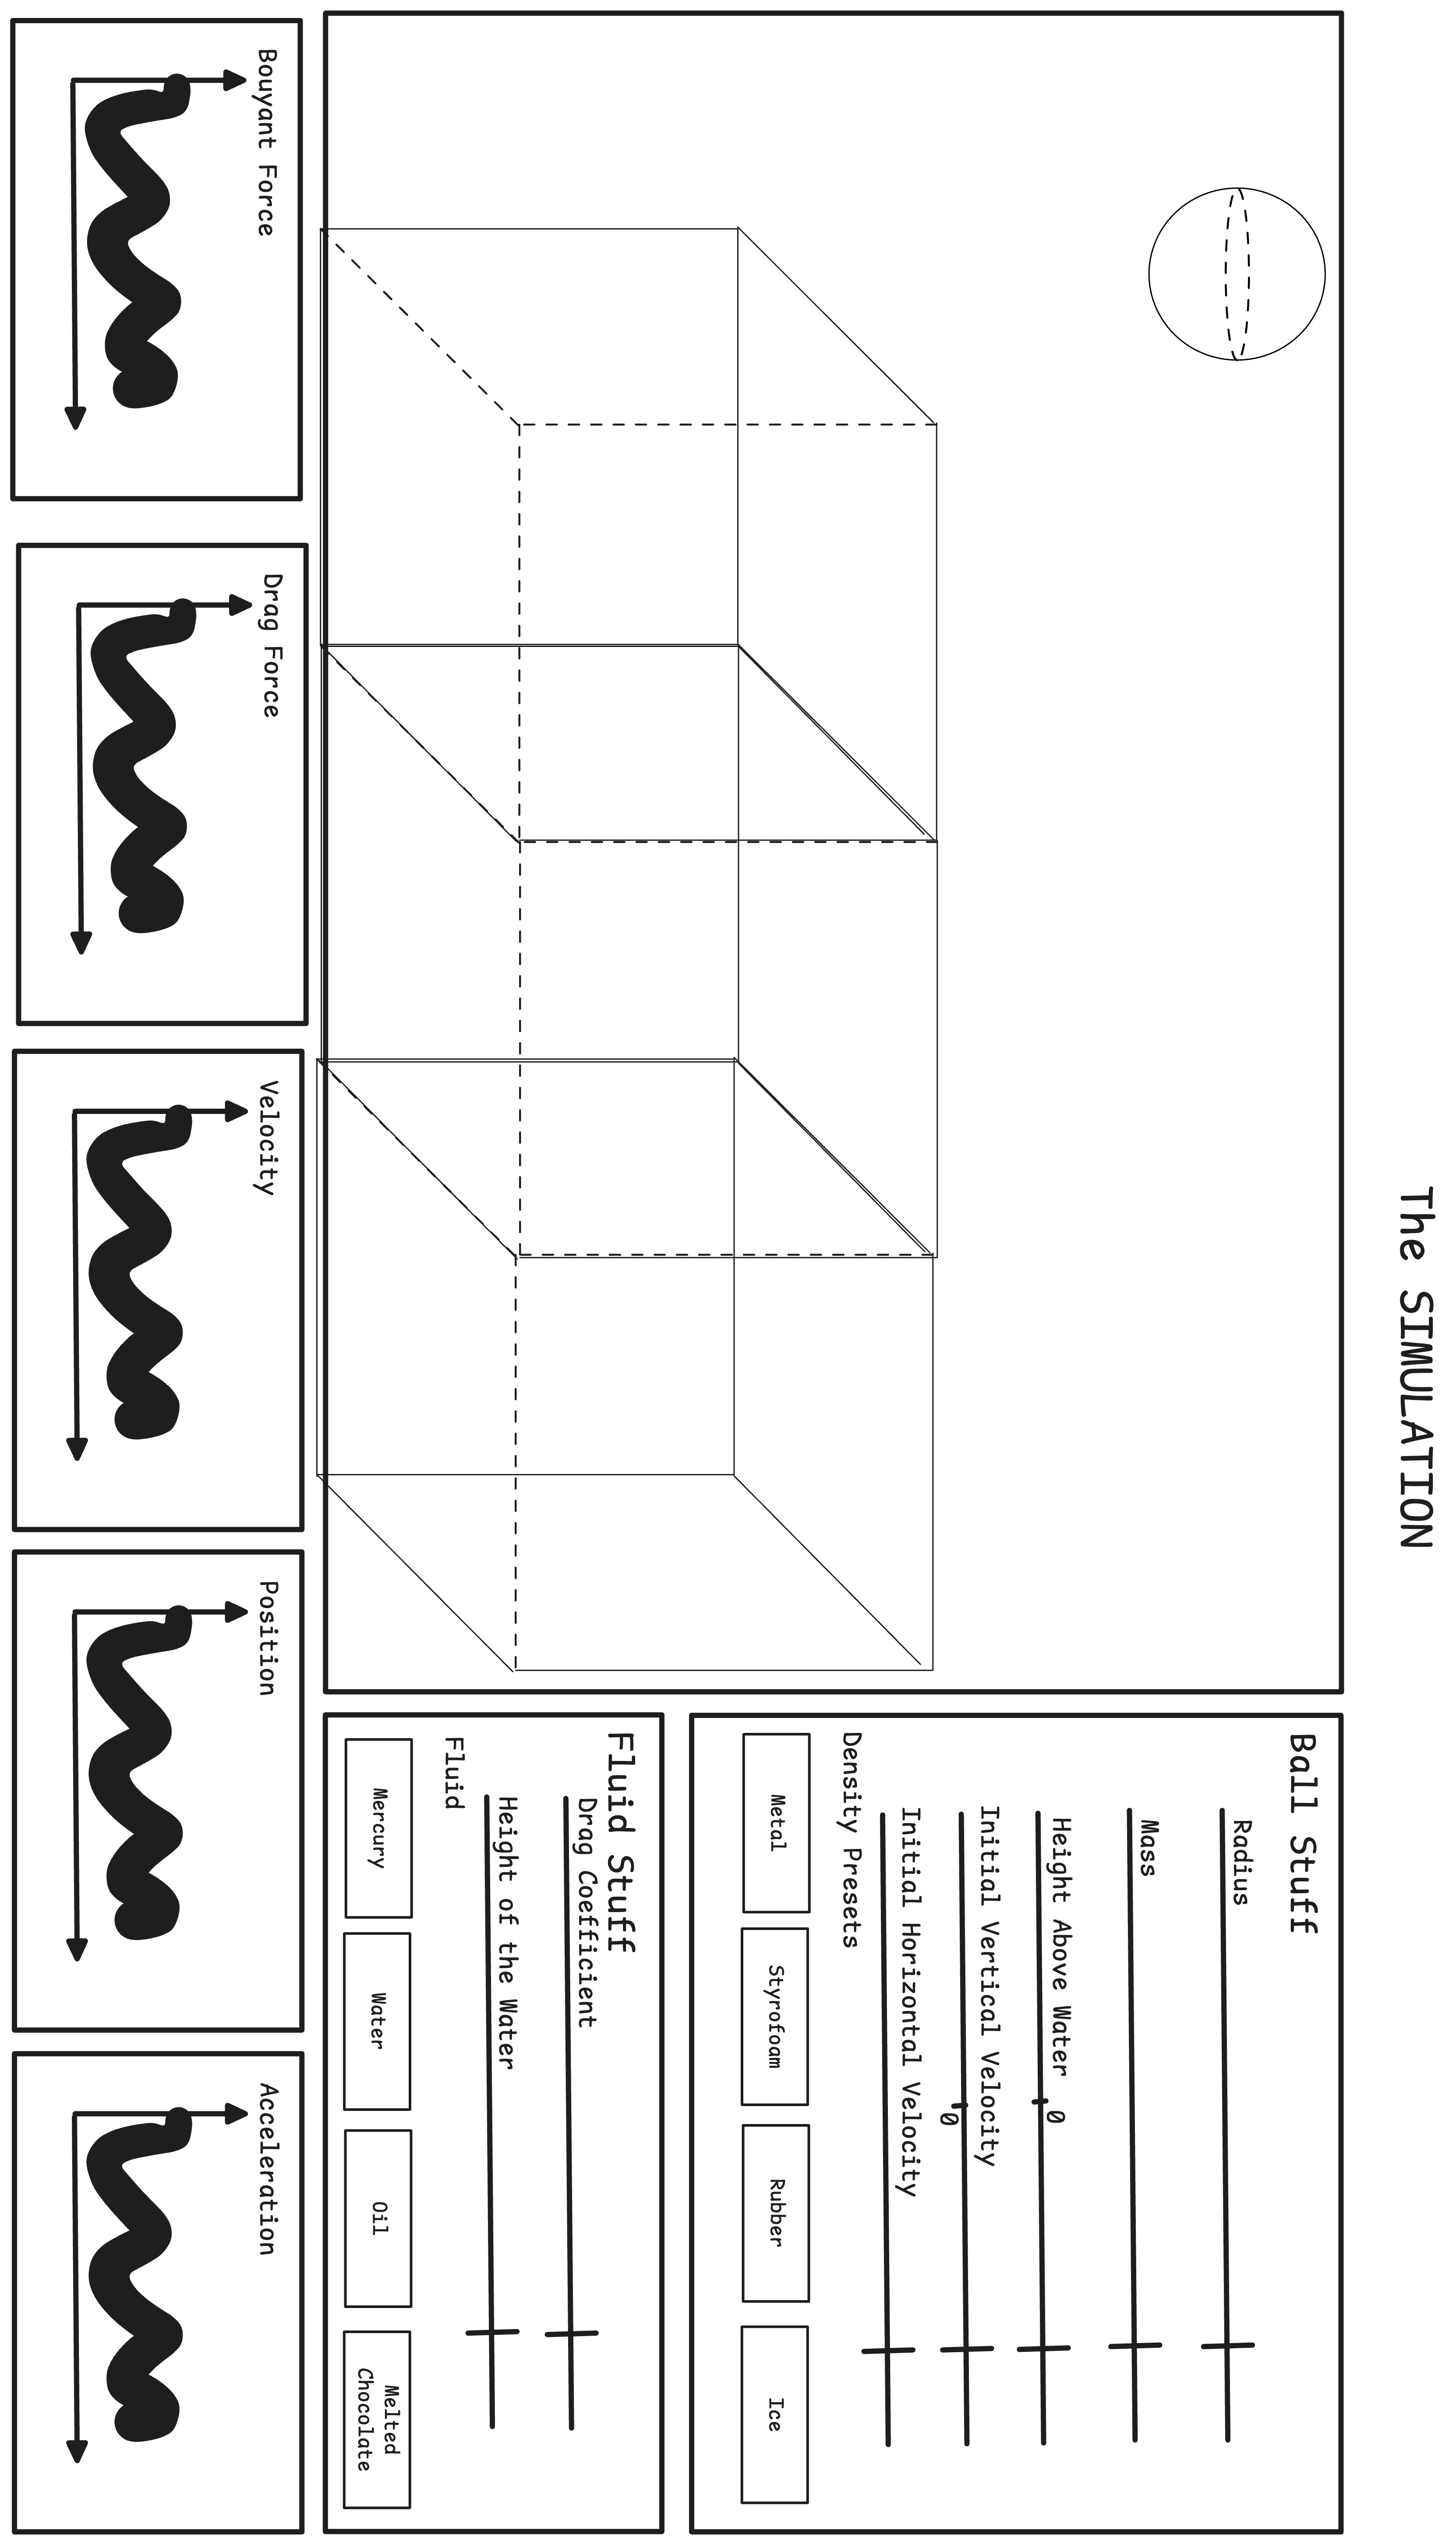
\includegraphics[width=0.72\textwidth]{figures/SIM.png}
\end{figure}


\end{document}